\chapter{Overview}

\todo{briefly explain this section}


\section{The Raspberry Pi 4 Cluster} \label{pi4cluster}

\todo{talk and show a picture of the physical testbed}

\begin{table}[H]
    \centering
    \begin{tabular}{ |p{4cm}||p{2cm}|p{3cm}|p{2cm}|p{2cm}|p{2cm}|  }
        \hline
        \multicolumn{6}{|c|}{\textbf{Raspberry Pi 4 Specifications}} \\
        \hline
        CPU & RAM & NICs & Storage & USB & OS\\
        \hline
        Broadcom BCM2711 \newline Cortex-A72 (ARMv7-rev3) 64-bit SoC \newline 1.5GHz, Quad-core &
        4GB LPDDR4-2400 SDRAM &
        Gigabit Ethernet Controller (part of CPU) \newline \newline Dual IEEE 802.11ac WiFi 5, Bluetooth 5.0, BLE &
        32GB Micro-SD &
        2 USB 3.0 ports \newline 2 USB 2.0 ports &
        Raspbian Buster (Linux)\\
        \hline
    \end{tabular}
    \caption{The hardware specifications of Raspberry Pi 4.}
\end{table}


\section{Network Topology} \label{topology}

\todo{talk and show a diagram of the network topology}

\begin{figure}[H]
    \centering
    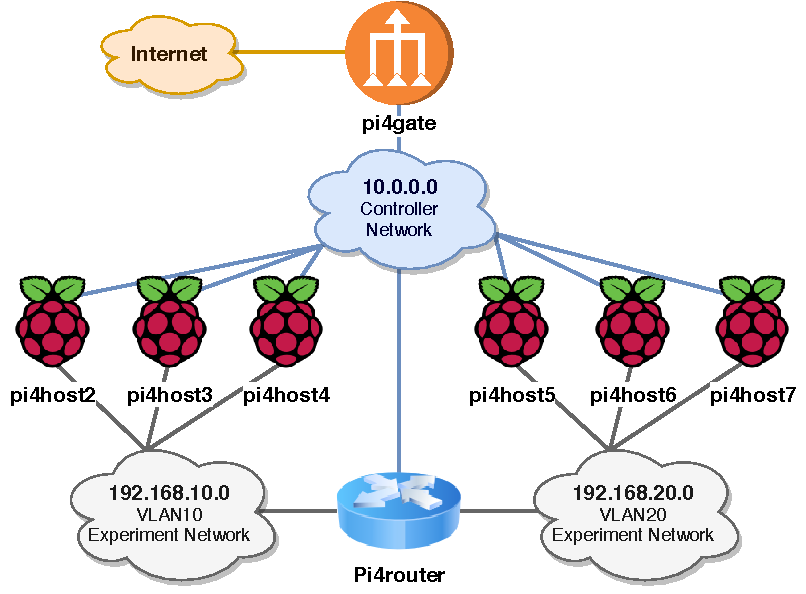
\includegraphics[width=0.6\linewidth]{network_topology}
    \captionsetup{width=0.6\linewidth}
    \caption{The logical network topology for the Raspberry Pi 4 cluster testbed. \todo{maybe update diagram to account for virtual interfaces and VLANs}}
    \label{fig:network_topology}
\end{figure}